\documentclass[12pt]{article}
\usepackage{graphicx} % Required for inserting images
\usepackage{hyperref}
\usepackage{polski}
\usepackage[utf8]{inputenc}
\usepackage[dvipsnames]{xcolor}
\usepackage{listings}
\usepackage{algorithm}
\usepackage{algpseudocode}
\usepackage{amsthm}
\usepackage{amsmath}
\usepackage[margin=1in]{geometry}
\usepackage{tikz}
\usepackage{float} % no replacements

\theoremstyle{definition}
\newtheorem{definition}{Definicja}[section]

\newcommand\YAMLcolonstyle{\color{red}\mdseries}
\newcommand\YAMLkeystyle{\color{black}\bfseries}
\newcommand\YAMLvaluestyle{\color{blue}\mdseries}

\theoremstyle{definition}
\newtheorem{example}{Przykład}[section]

\makeatletter

\newcommand\ProcessThreeDashes{\llap{\color{cyan}\mdseries-{-}-}}

\title{ Wprowadzenie do sztucznej inteligencji --- Automatyczne tworzenie drzewa decyzyjnego z tablicy decyzyjnej }
\author{Dmytro Tolstoi, Oleh Kiprik, Andrii Voznesenskyi}
\date{Semestr 2024L}

\begin{document}

\maketitle
\newpage

\setcounter{section}{0}
\section{Wstęp}

Sztuczna inteligencja (SI) jest dynamicznie rozwijającą się dziedziną informatyki, która naśladuje zdolności poznawcze ludzi, umożliwiając maszynom uczenie się, rozumowanie i rozwiązywanie problemów. Wśród wielu zastosowań SI, systemy wspomagania decyzji (DSS) odgrywają kluczową rolę w dostarczaniu niezbędnych narzędzi i metodologii, które pomagają w podejmowaniu skomplikowanych decyzji biznesowych, technicznych czy naukowych. Podstawą działania wielu z tych systemów są algorytmy bazujące na strukturach danych takich jak tablice i drzewa decyzyjne.

\begin{definition}
Tablica decyzyjna jest matematyczną abstrakcją służącą do reprezentowania i analizowania decyzji. Składa się z wierszy reprezentujących możliwe scenariusze lub przypadki, kolumn symbolizujących atrybuty lub warunki, oraz decyzji wynikających z kombinacji tych warunków. Rzetelną definicją względem także i przetrzeni hipotez można uzyskać z \cite{kohavi1995power}.
\end{definition}

\begin{example}
    
Przykładowa tablica decyzyjna reprezentującą decyzje dotyczące wyjścia na spacer w zależności od pogody:

\begin{table}[h]
\centering
\begin{tabular}{|c|c|c|}
\hline
Pogoda & Temperatura & Decyzja \\
\hline
Słonecznie & Ciepło & Wyjdź \\
Słonecznie & Zimno & Nie wychodź \\
Deszczowo & Ciepło & Nie wychodź \\
Deszczowo & Zimno & Nie wychodź \\
\hline
\end{tabular}
\caption{Tablica decyzyjna dla wyjścia na spacer}
\end{table}

\end{example}

\begin{definition}
Drzewo decyzyjne to graficzna reprezentacja procesu decyzyjnego, gdzie każdy węzeł wewnętrzny reprezentuje test na atrybucie, każda gałąź to wynik testu, a każdy liść to etykieta klasy. Drzewa decyzyjne są wykorzystywane w wielu dziedzinach do wsparcia procesu decyzyjnego, dzięki ich zdolności do modelowania złożonych procesów decyzyjnych w sposób intuicyjny i łatwy do interpretacji.
\end{definition}

\begin{definition}
    Funkcji testów rozróżniamy na 2 klasy:
    \begin{itemize}
        \item Testy operują się na wartościach pojedyńczego atrybutu:\[
        t: V_a \rightarrow R_t
        \]
        \item Testy będące kombinacją wartości kilku atrybutów: 
        \[
        t: V_{a_1} \times V_{a_2} \times \ldots \times V_{a_k} \rightarrow R_t
        \]
    \end{itemize}
    gdzie
    \begin{itemize}
        \item $V_a$ : dziedzina atrybutu $a$
        \item $R_t$ : zbiór możliwych wyników testu
    \end{itemize}
\end{definition}

\begin{example}
    Przykładowymi funkcjami testów z Tablicy 1 mogą być:
    \begin{itemize}
        \item $t(x) \rightarrow a_i(x)$, czyli dla pierwszego wiersza i atrybutu \textbf{Temperatura} wynikiem będzie \textbf{Ciepło} (test tożsamościowy).
        \item $t(x) = 
        \begin{cases}
            1 & \textrm{if } (a_i(x) = v)\\
            0 & \textrm{otherwise}
        \end{cases}$, to znaczy, że jeżeli $v =$ \textbf{Zimno}, to dla pierwszego wiersza wynik będzie 0, dla drugiego 1 (test równościowy).
        \item z poprzedniego testu możemy założyć, że $v$ nie jest pojędyńczym elementem, a jest zbiorem zadowalających atrybutów $V$ i zamieniając warunek na $a_i(x)\in V$ otrzymujemy test przynależnościowy.
    \end{itemize}
\end{example}

\begin{definition}
    Każdy zbiór obiektów $X$ ulega podziale na klasy decyzyjne:
    \[
    X = C_1 \cup C_2 \cup \ldots \cup C_d
    \]
    gdzie $C_i = \{u \in X: decision(u) = i\}$. To znaczy, że klasą decyzyjną $C_i$ nazywamy taki podzbiór $X$, w którym każdy obiekt z tego podzbioru przyjmuje decyzję $i$. Dodatkowo, potrzebujemy narzędzi do analizy tych klas:
    \[
    Conflict(X)=\sum_{i < j}|C_i|\times|C_j|=\frac{1}{2}\left(|X|^2-\sum|C_i|^2\right)
    \]
    \[
    Entropy(X) = -\sum\frac{|C_i|}{|X|}\log{\frac{|C_i|}{|X|}}
    \]

    Funkcja $Conflict(X)$ oraz $Entropy(X)$ przyjmują,
    \begin{itemize}
        \item największą, wartość, gdy rozkład klas decyzyjnych w
zbiorze $X$ jest równomierny.
        \item najmniejszą wartość, gdy wszystkie obiekty w $X$ są
jednej kategorii ($X$ jest \textbf{jednorodny})
    \end{itemize}
\end{definition}



\begin{example}
    Tablica 1 ma dwie klasy: $C_{\textrm{wyjdź}}=\{\{\textrm{Słonecznie, Ciepło}\}\}$ i 

$C_{\textrm{nie wychodź}}=\{\{\textrm{Słonecznie, Zimno}\},\{\textrm{Deszczowo, Ciepło}\},\{\textrm{Deszczowo, Zimno}\}\}$.
\end{example}


\section{Algorytm tworzenia drzewa decyzyjnego z tablicy decyzyjnej}

Algorytm prezentowany w dalszej części pracy skupia się na automatycznym tworzeniu drzewa decyzyjnego z tablicy decyzyjnej, co jest fundamentalnym procesem w budowaniu efektywnych i skutecznych systemów wspomagania decyzji. Proces ten wymaga starannej analizy i przetwarzania danych wejściowych, aby zbudować strukturę drzewa, która najlepiej oddaje zależności między atrybutami a decyzjami w danych.

\begin{algorithm}[H]
\caption{Tworzenie drzewa decyzyjnego z tabeli decyzyjnej. \textbf{Opis algorytmu:} Algorytm \textit{BudujDrzewo} rozpoczyna od sprawdzenia, czy wszystkie dane w zbiorze należą do tej samej klasy. Jeśli tak, tworzy węzeł liścia z dominującą klasą. W przeciwnym przypadku algorytm wybiera najlepszy atrybut do podziału danych, tworzy węzeł decyzyjny i rekurencyjnie buduje poddrzewa dla każdej wartości najlepszego atrybutu. Proces ten kontynuowany jest do osiągnięcia określonej głębokości drzewa lub do momentu, gdy nie ma więcej atrybutów do podziału lub wszystkie pozostałe dane należą do tej samej klasy. 
Funkcja \textsc{WszystkieTakieSame} sprawdza jednorodność klasy wszystkich elementów w zbiorze danych. Jeżeli wszystkie elementy należą do tej samej klasy, funkcja zwraca wartość \textit{prawda}; w przeciwnym razie zwraca \textit{fałsz}. Funkcja \textsc{NowyWęzeł} tworzy nowy węzeł drzewa decyzyjnego. Dla węzłów liści, argumentem jest etykieta klasy, natomiast dla węzłów wewnętrznych jest to atrybut, według którego następuje podział. Funkcja \textsc{Filtruj} przyjmuje zbiór danych oraz atrybut z jego wartością i zwraca nowy zbiór danych zawierający tylko te rekordy, które mają daną wartość dla wybranego atrybutu. Funkcja \textsc{DodajDziecko} przyjmuje dwa argumenty: węzeł nadrzędny oraz węzeł, który ma zostać dodany jako dziecko. Funkcja włącza nowy węzeł do struktury drzewa jako potomka węzła nadrzędnego.}\label{alg:decision_tree}
\begin{algorithmic}[1]
\Procedure{BudujDrzewo}{\emph{Dane}, \emph{Atrybuty}, \emph{Głębokość}}
    \If{\textsc{WszystkieTakieSame}(Dane)}
        \State \textbf{return} \textsc{NowyWęzeł}(Klasa=dominująca klasa w $Dane$)
    \EndIf
    \If{$Atrybuty = \emptyset$ \textbf{or} \emph{Głębokość} $ = 0$}
        \State \textbf{return} \textsc{NowyWęzeł}(Klasa=najczęstsza klasa w $Dane$)
    \EndIf
    \State $NajlepszyAtrybut \gets \textsc{WybierzNajlepszyAtrybut}(Dane, Atrybuty)$
    \State $\textsc{Węzeł} \gets \textsc{NowyWęzeł}(Klasa=NajlepszyAtrybut)$
    \ForAll{\emph{wartość} $\in \textsc{Wartości}(NajlepszyAtrybut)$}
        \State $PodDane \gets \textsc{Filtruj}(Dane, NajlepszyAtrybut,$ \emph{wartość)}
        \If{$PodDane = \emptyset$}
            \State \textsc{DodajDziecko}($\textsc{Węzeł}$, \textsc{NowyWęzeł}(Klasa=najczęstsza klasa w $Dane$))
        \Else
            \State \textsc{DodajDziecko}($\textsc{Węzeł}$, \textsc{BudujDrzewo}($PodDane, Atrybuty \setminus{NajlepszyAtrybut}, $\emph{Głębokość}$-1$))
        \EndIf
    \EndFor
    \State \textbf{return} \textsc{Węzeł}
\EndProcedure
\end{algorithmic}
\end{algorithm}

\textbf{Dowód poprawności algorytmu \textit{BudujDrzewo}:}

Algorytm \textit{BudujDrzewo} można uznać za poprawny na podstawie indukcji matematycznej. Dla zbioru danych, który w całości należy do jednej klasy, algorytm natychmiast zwraca węzeł liścia z tą klasą, co jest oczywiście poprawnym drzewem decyzyjnym dla tego przypadku bazowego.

Załóżmy teraz, że algorytm działa poprawnie dla wszystkich zbiorów danych o wielkości mniejszej niż $n$. Dla zbioru danych o wielkości $n$, jeśli nie wszystkie elementy należą do tej samej klasy, algorytm wybiera atrybut, który najlepiej dzieli zbiór danych (na podstawie kryterium, takiego jak zysk informacji). Następnie, algorytm rekurencyjnie buduje poddrzewa dla każdej wartości tego atrybutu na podzbiorach danych, które są mniejsze niż zbiór początkowy. Na podstawie założenia indukcyjnego, te rekurencyjne wywołania zwracają poprawne poddrzewa. Stąd, sklejenie tych poddrzew z węzłem decyzyjnym dla wybranego atrybutu również musi dać poprawne drzewo decyzyjne dla całego zbioru danych.

Ponieważ algorytm działa poprawnie dla przypadku bazowego i, zakładając poprawność dla przypadków mniejszych niż $n$, jest poprawny dla przypadku $n$, na mocy indukcji matematycznej algorytm \textit{BudujDrzewo} jest poprawny dla wszystkich wielkości zbiorów danych.

\section{Wybór testu}
W algorytmie nie zostało opisano w jaki sposób będziemy wybierali najlepszy atrybut, w tej części spróbujemy pokazać narzędzia do rozwiązania tego probemu. 

Kontynuując \cite{felicjawsi}, niech $t$ definiuje podział $X$ na podzbiory: $X_1 \cup \ldots \cup X_r$. Możemy stosować następujące miary do oceniania testów:
    \begin{itemize}
        \item liczba par obiektów rozróżnionych przez test $t$ (Rożróżnialność).
        \[
        disc(t,X) = Conflict(X) - \sum Conflict(X_i)
        \]
        \item kryterium przyrostu informacji
        \[
        Gain(t,X)=Entropy(X) - \sum_i \frac{|X_i|}{|X|}Entropy(X_i)
        \]
    \end{itemize}

    Im większe są wartości tych ocen, tym lepszy jest test.

    Również do oceny testów możemy wykorzystać współczynnik przyrostu informacji zamiast bezwzględnego przyrostu inforamcji: 
    \[
    Gain\_ratio=\frac{Gain(t,X)}{iv(t,X)}
    \]
    gdzie $iv(t,X)$, zwana wartością informacyjną testu $t$, jest zdefiniowana jak: \[
    iv(t,X)= -\sum \frac{X_i}{X}\log \frac{X_i}{X}
    \]

\section{Konwersja na drzewo decyzyjne}

Na podstawie powyższej tablicy decyzyjnej, możemy stworzyć następujące drzewo decyzyjne (przykład powstał w rzeczywistego przykładu ukłądu uproszczonego z pozycji \cite{magee1964decision}.):
\begin{enumerate}
    \item Rozpoczynamy od węzła początkowego, który reprezentuje cały zbiór danych i dzielimy go na podstawie atrybutu, który zapewnia najlepszą separację (w tym przypadku "Pogoda").
    \item Dla każdej wartości atrybutu "Pogoda" (Słonecznie, Deszczowo) tworzymy gałąź i decydujemy o kolejnym podziale lub kończymy w liściu z decyzją ("Wyjdź", "Nie wychodź").
    \item Proces kontynuujemy rekurencyjnie dla każdej gałęzi, aż wszystkie rekordy w gałęzi będą należały do tej samej klasy decyzyjnej lub osiągniemy maksymalną głębokość drzewa
\end{enumerate}
\begin{figure}[H]
\centering
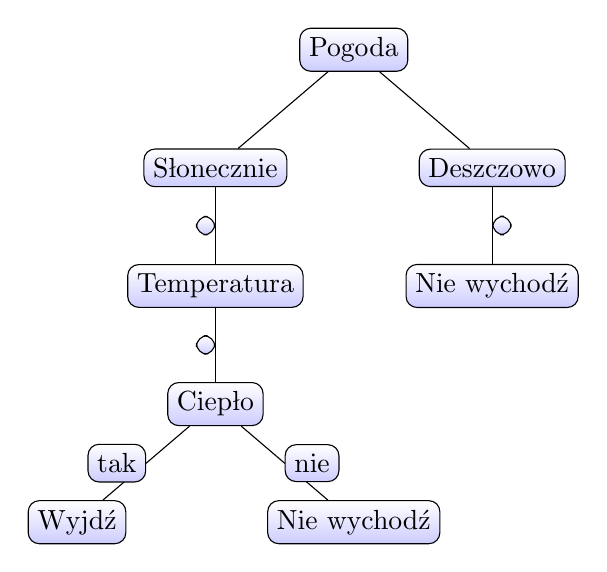
\begin{tikzpicture}[sibling distance=10em,
  every node/.style = {shape=rectangle, rounded corners,
    draw, align=center,
    top color=white, bottom color=blue!20}]]
  \node {Pogoda}
    child { node {Słonecznie} 
      child { node {Temperatura} 
        child { node {Ciepło} 
          child { node {Wyjdź} edge from parent node[left] {tak} } 
          child { node {Nie wychodź} edge from parent node[right] {nie} }
          edge from parent node[left] {} 
        } 
        edge from parent node[left] {} 
      }
    }
    child { node {Deszczowo}
      child { node {Nie wychodź} edge from parent node[right] {} }
    };
\end{tikzpicture}
\caption{Drzewo decyzyjne dla wyjścia na spacer}
\end{figure}

Jak widać, drzewo decyzyjne pozwala nam w prosty i intuicyjny sposób zobrazować proces decyzyjny oparty na tablicy decyzyjnej. 


% \section*{Eksperymenty i wyniki}

% \section*{Opis eksperymentów}

% \section*{Analiza wyników}

% \section*{Podsumowanie i wnioski}
% \addcontentsline{toc}{chapter}{Podsumowanie i wnioski}

% \section*{Podsumowanie}


\bibliographystyle{plain}
\nocite{nguyen2000datamining}
\bibliography{references}


\end{document}